\documentclass[12pt]{article}
\usepackage{graphicx}
\usepackage{hyperref}
\usepackage{geometry}
\usepackage{longtable}
\usepackage{float}
\usepackage{tikz}

\geometry{a4paper, margin=1in}

\title{Software Design Specification \\ \large Real-Time Safety Monitoring System for Industrial Workplaces}
\author{Syed Ahad Ali, Asad Ullah Chaudhry, Muhammad Arsalan Hussain, \\ Muzzammil Kamran Sattar}
\date{\today}

\begin{document}

\maketitle
\tableofcontents
\newpage

\section{Introduction}
This document outlines the Software Design Specification (SDS) for the Real-Time Safety Monitoring System designed for Dawlence’s sheet metal plant in Karachi. It expands upon the system requirements specified in the SRS document by describing how the software requirements will be implemented. This SDS will provide a detailed overview of the system architecture, data model, data pipeline, and technical implementation.

\section{Project Architecture (30 Points)}
\subsection{System Overview}
The system comprises the following major components:
\begin{itemize}
    \item \textbf{CCTV Cameras:} Capture real-time footage across factory zones.
    \item \textbf{YOLO Models:} Process video frames for safety hazard detection.
    \item \textbf{Backend Server:} Coordinates communication between system components and manages data storage.
    \item \textbf{Web-Based Dashboard:} Visualizes hazard notifications and safety analytics.
    \item \textbf{Notification System:} Delivers alerts via dashboard, email, and SMS.
\end{itemize}

\begin{figure}[h]
    \centering
    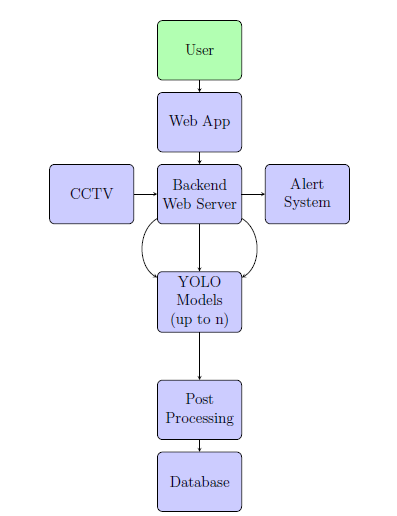
\includegraphics[scale = 0.8]{system_block.png}
    \caption{System Block Diagram}
\end{figure}
Fig.1  shows how inputs and outputs are processed through the system.
The system recieves input from CCTV cameras, processes it through the YOLO models, 
and stores the data in the backend server. The web-based dashboard visualizes an annotated
view of the CCTV input (annotations done by deep learning models) as well as
presents the user with statistics of past hazard detections (created using stored data) 
The notification system alerts relevant personnel of any detected hazards. Currently, the notification system is an automated
email to the supervisor as well as a desktop notification to the dashboard user.



\begin{figure}[h]
    \centering
    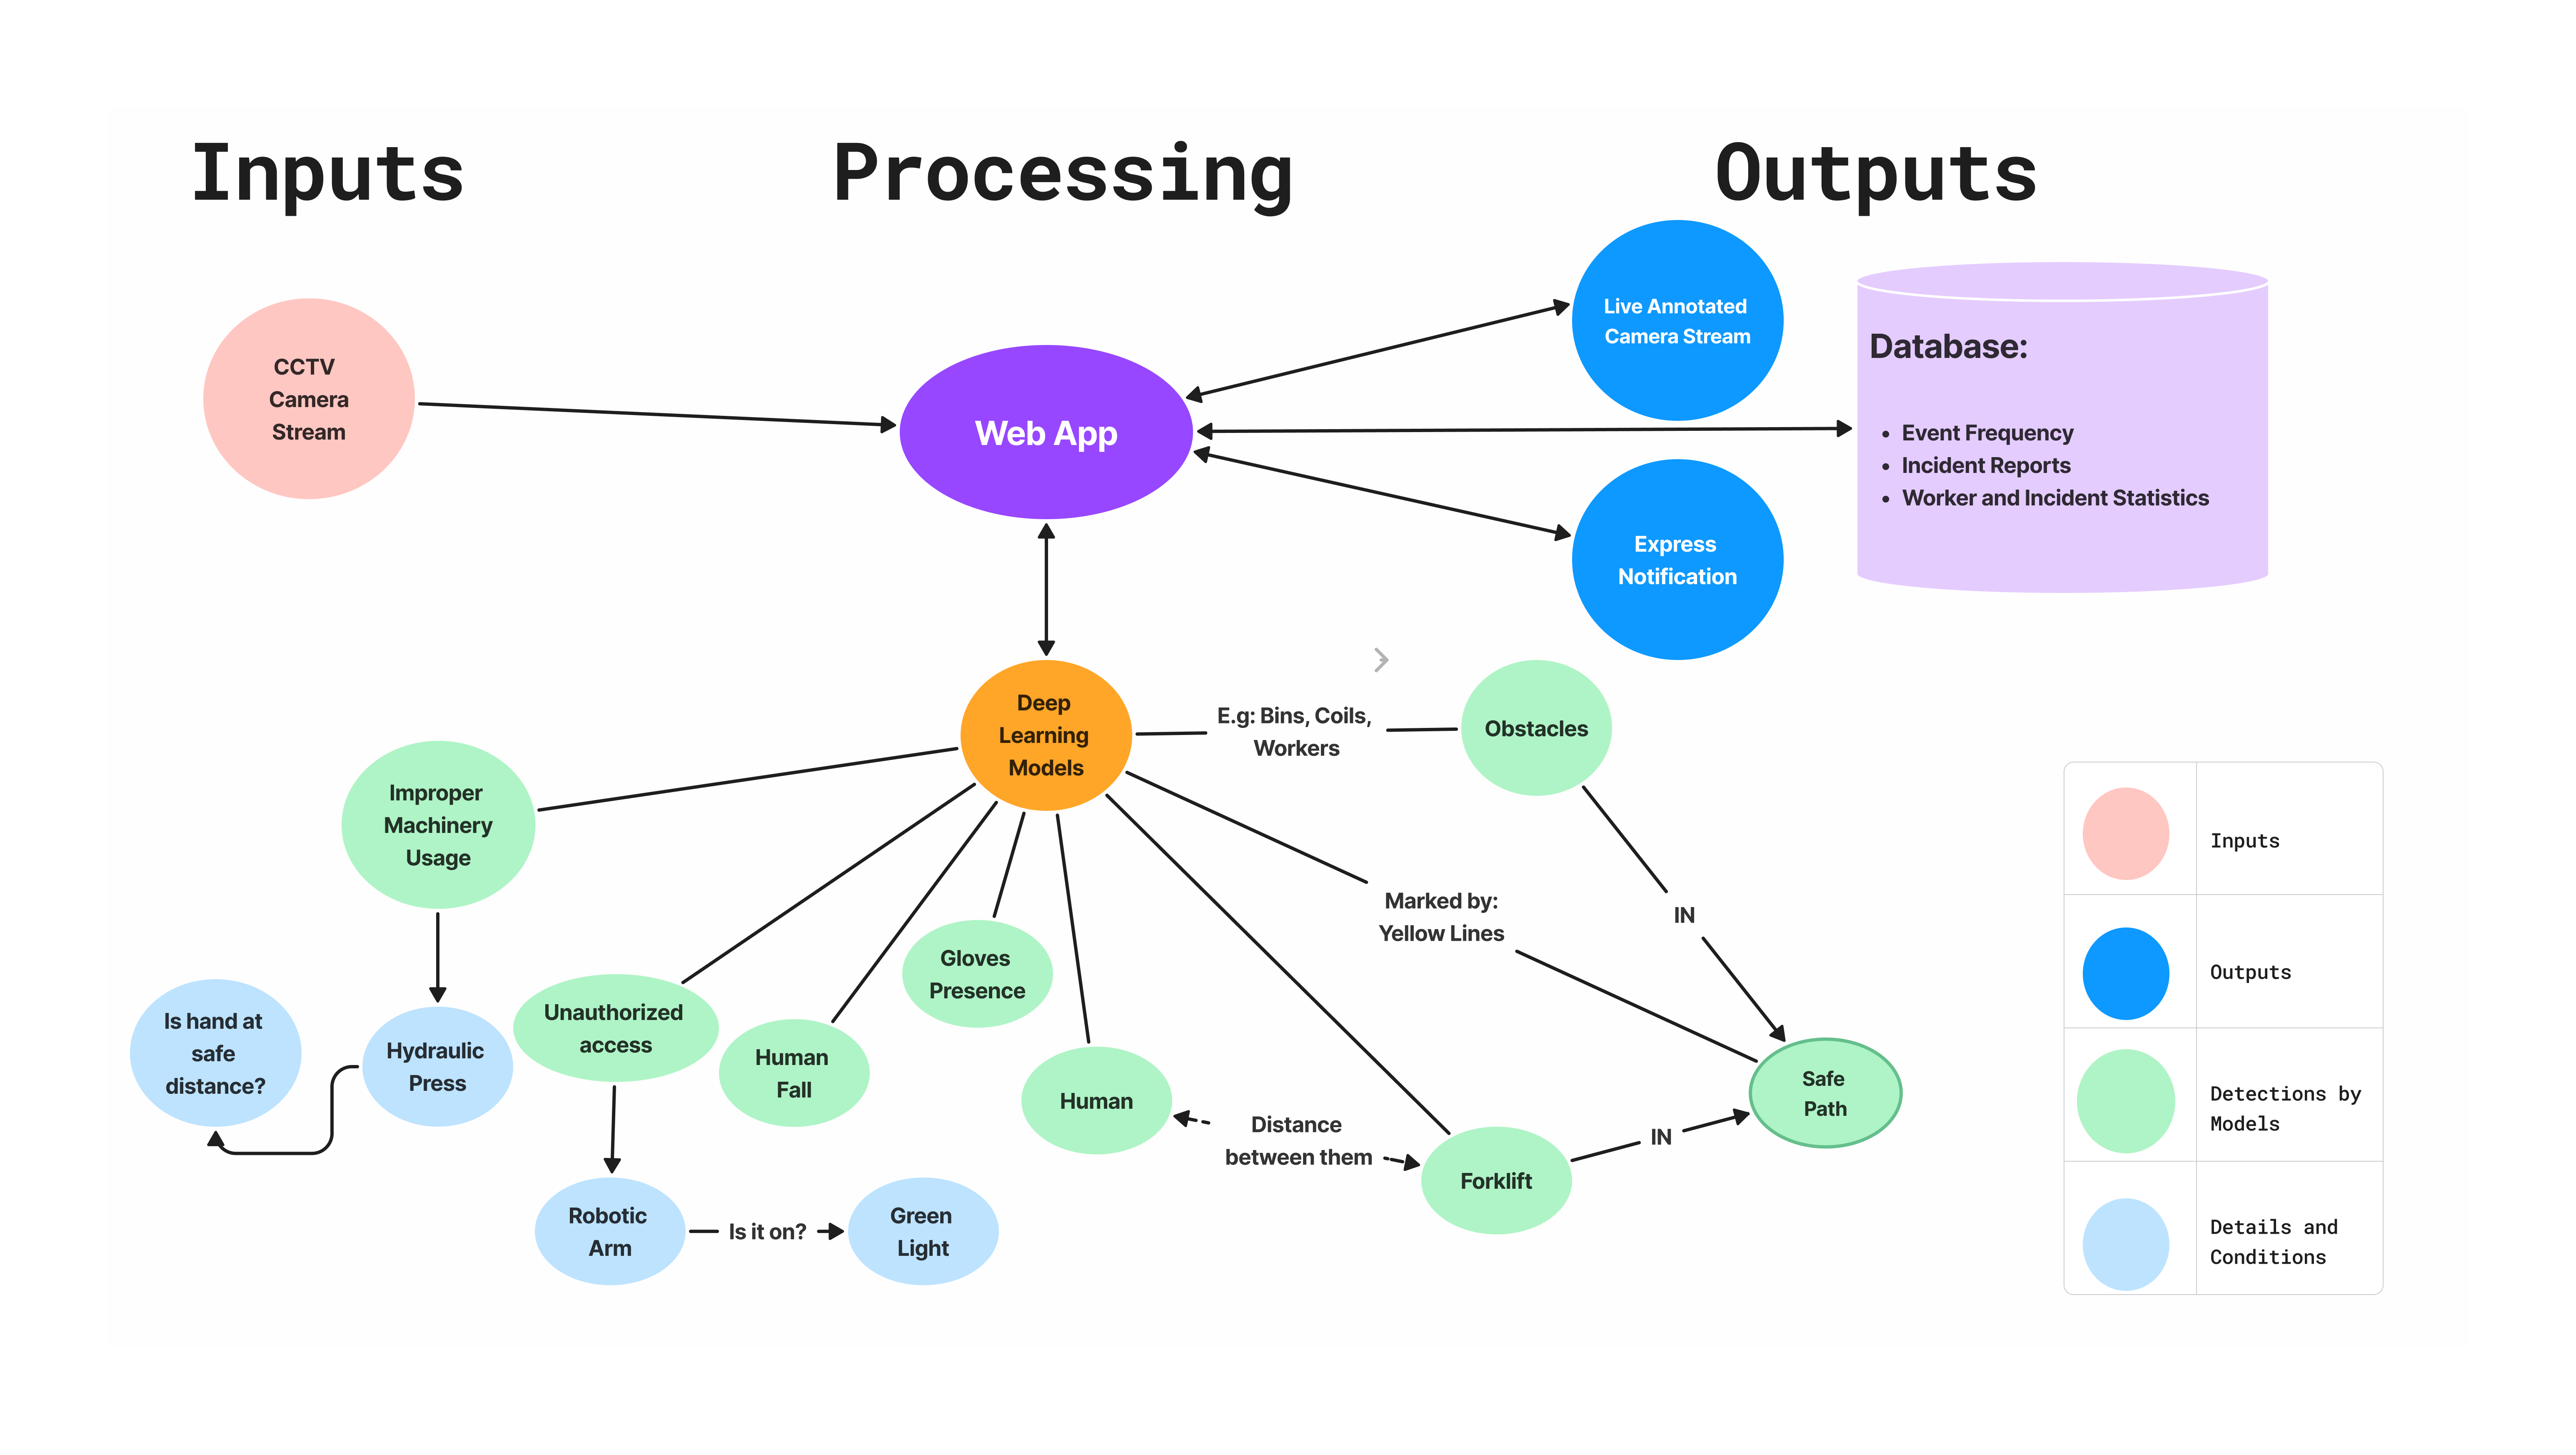
\includegraphics[width=\textwidth]{system_flow.png}
    \caption{System Flow Diagram}
\end{figure}
Fig.2 shows a more detailed view of each detection and when they're triggered. 
Once our system recieves the CCTV footage, YOLO models analyse it frame by frame
to detect the presence and location (in pixel coordinates) of people, forklifts,
bare hands, and obstacles. 

The models detect the following objects (for the given reasons):
\begin{itemize}
    \item \textbf{People:} 
    \begin{itemize}
        \item Fall detection
        \item Entry of restricted areas
        \item Safe distance between forklift and workers
        \item Improper machinery usage (e.g., standing on conveyor belts)
    \end{itemize}
    \item \textbf{Forklifts:}
    \begin{itemize}
        \item Speeding
        \item Proximity to workers
        \item Adherence to designated paths
    \end{itemize}
    \item \textbf{Bare Hands:} To check for PPE compliance.
    \item \textbf{Obstacles:} To check for path obstructions.

\end{itemize}
The safe paths and restricted areas are pre-defined as per Dawlence requirement. 


\newpage
\section{Data Model (25 Points)}
\subsection{Database Design}
The system database manages:
\begin{itemize}
    \item \textbf{Hazard Events:} Records details such as timestamp, camera location, hazard type, and alert status.
    \item \textbf{User Data:} Stores user roles and permissions for secure system access.
    \item \textbf{Video Metadata:} Tracks file locations and annotations for incident playback.
\end{itemize}

% \subsection{Entity-Relationship Diagram}
% \begin{figure}[h]
%     \centering
%     \includegraphics[width=\textwidth]{er_diagram_placeholder.png}
%     \caption{Entity-Relationship Diagram for Data Management}
%     \label{fig:er_diagram}
% \end{figure}

\subsection{Data Annotations}
Annotated data includes:
\begin{itemize}
    \item PPE compliance (e.g., gloves, shoes).
    \item Hazard zones and restricted area boundaries.
    \item Forklift proximity and speed.
\end{itemize}

\section{Data Pipeline}
\subsection{Training Data Pipeline}
\begin{figure}[H]
    \centering
    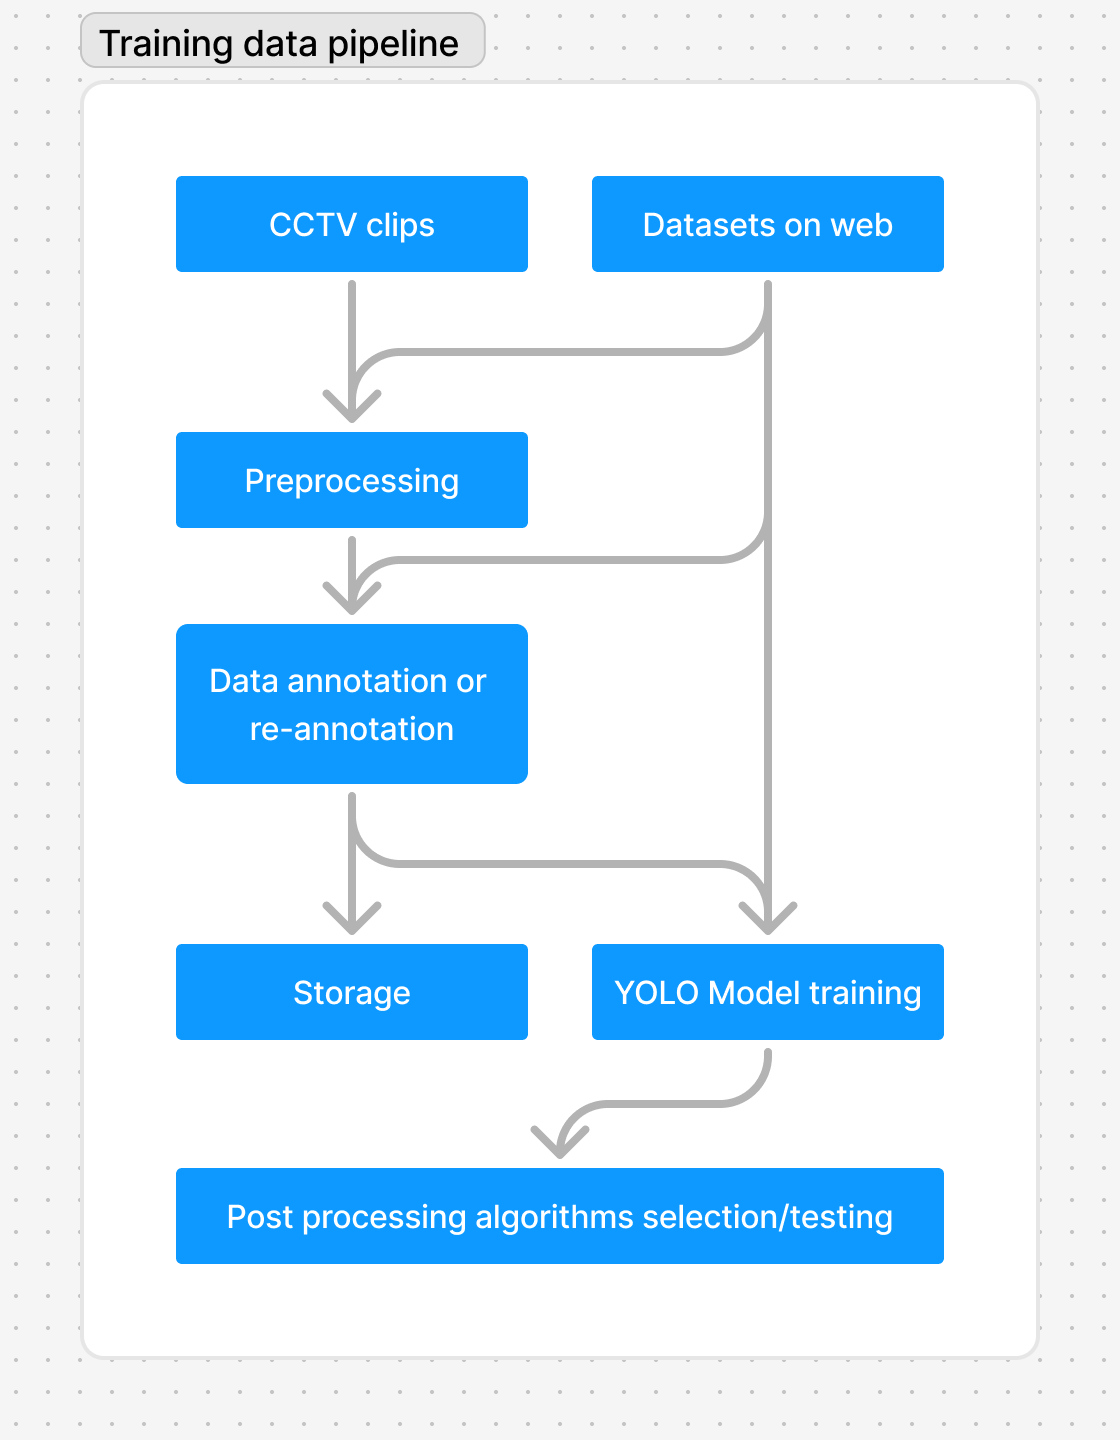
\includegraphics[width=0.75\textwidth]{training_pipeline.png}
    \caption{Training data pipeline diagram}
    \label{fig:pipeline1}
\end{figure}

\begin{enumerate}
    \item \textbf{Data Collection:} CCTV footage and publicly available datasets. Publicly available datasets may need to be preprocessed and/or re-annotated.
    \item \textbf{Preprocessing:} Frame extraction, resizing, and augmentation.
    \item \textbf{Data annotation:} Annotate frames manually.
    \item \textbf{YOLO Model Training:} Transfer learning on annotated datasets.    
    \item \textbf{Post-Processing algorithms testing:} Contextual filtering to detect hazards based on relationship of detecteions. Experiment with different methods to find most accurate for our purpose.
    \item \textbf{Storage:} Privately stored recording of CCTV clips, annotated frames and associated data.
\end{enumerate}

\subsection{Live Data Pipeline}
\begin{figure}[H]
    \centering
    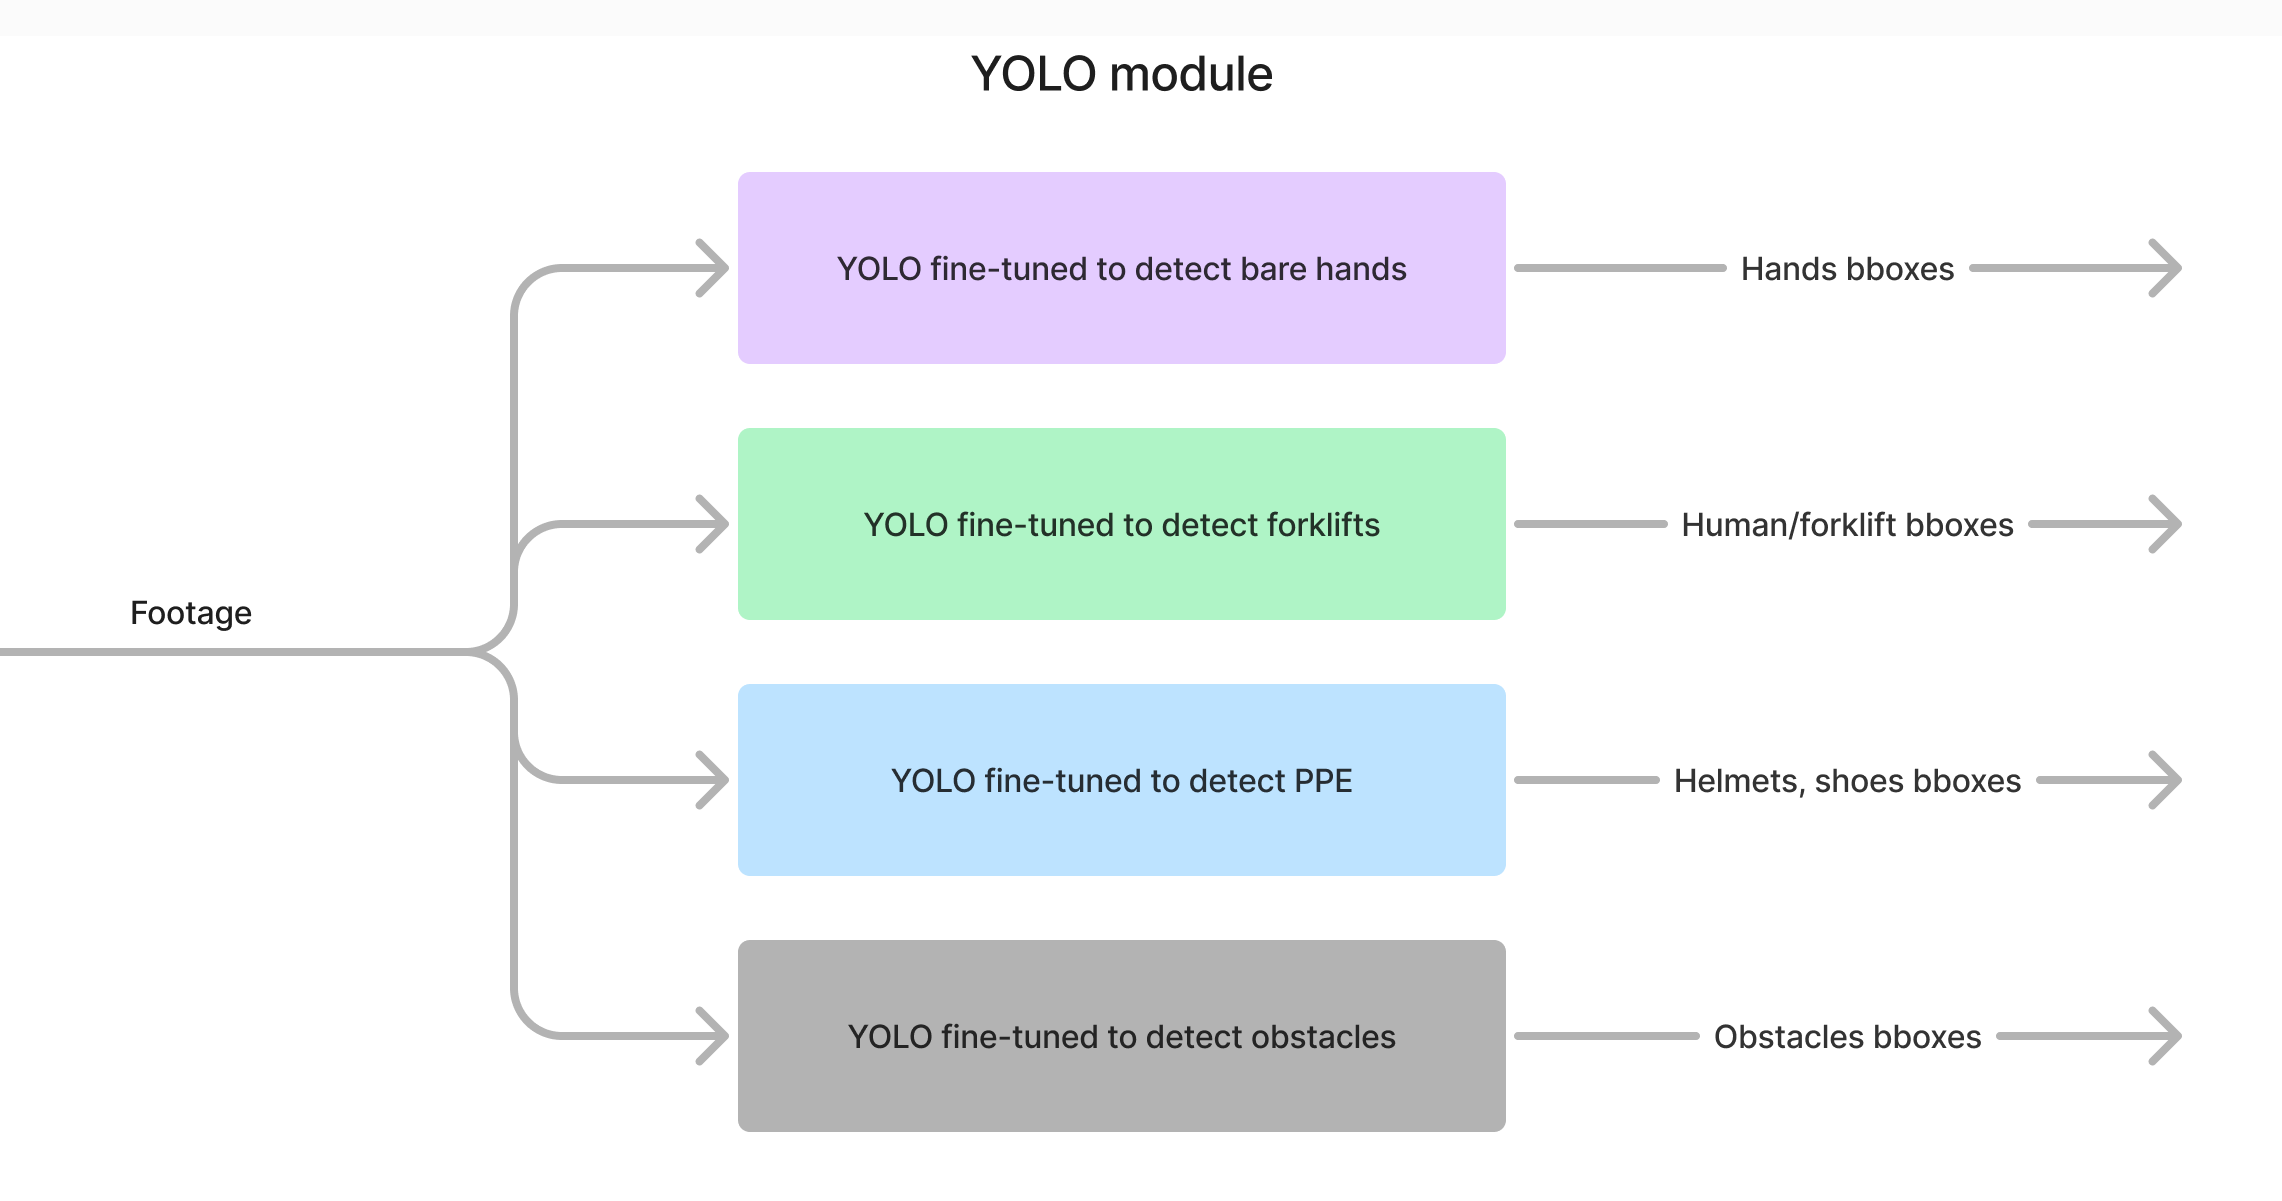
\includegraphics[width=\textwidth]{yolo_module.png}
    \caption{YOLO module: $\leq4$ YOLO models running in parallel}
    \label{fig:yolo}
\end{figure}

\begin{figure}[H]
    \centering
    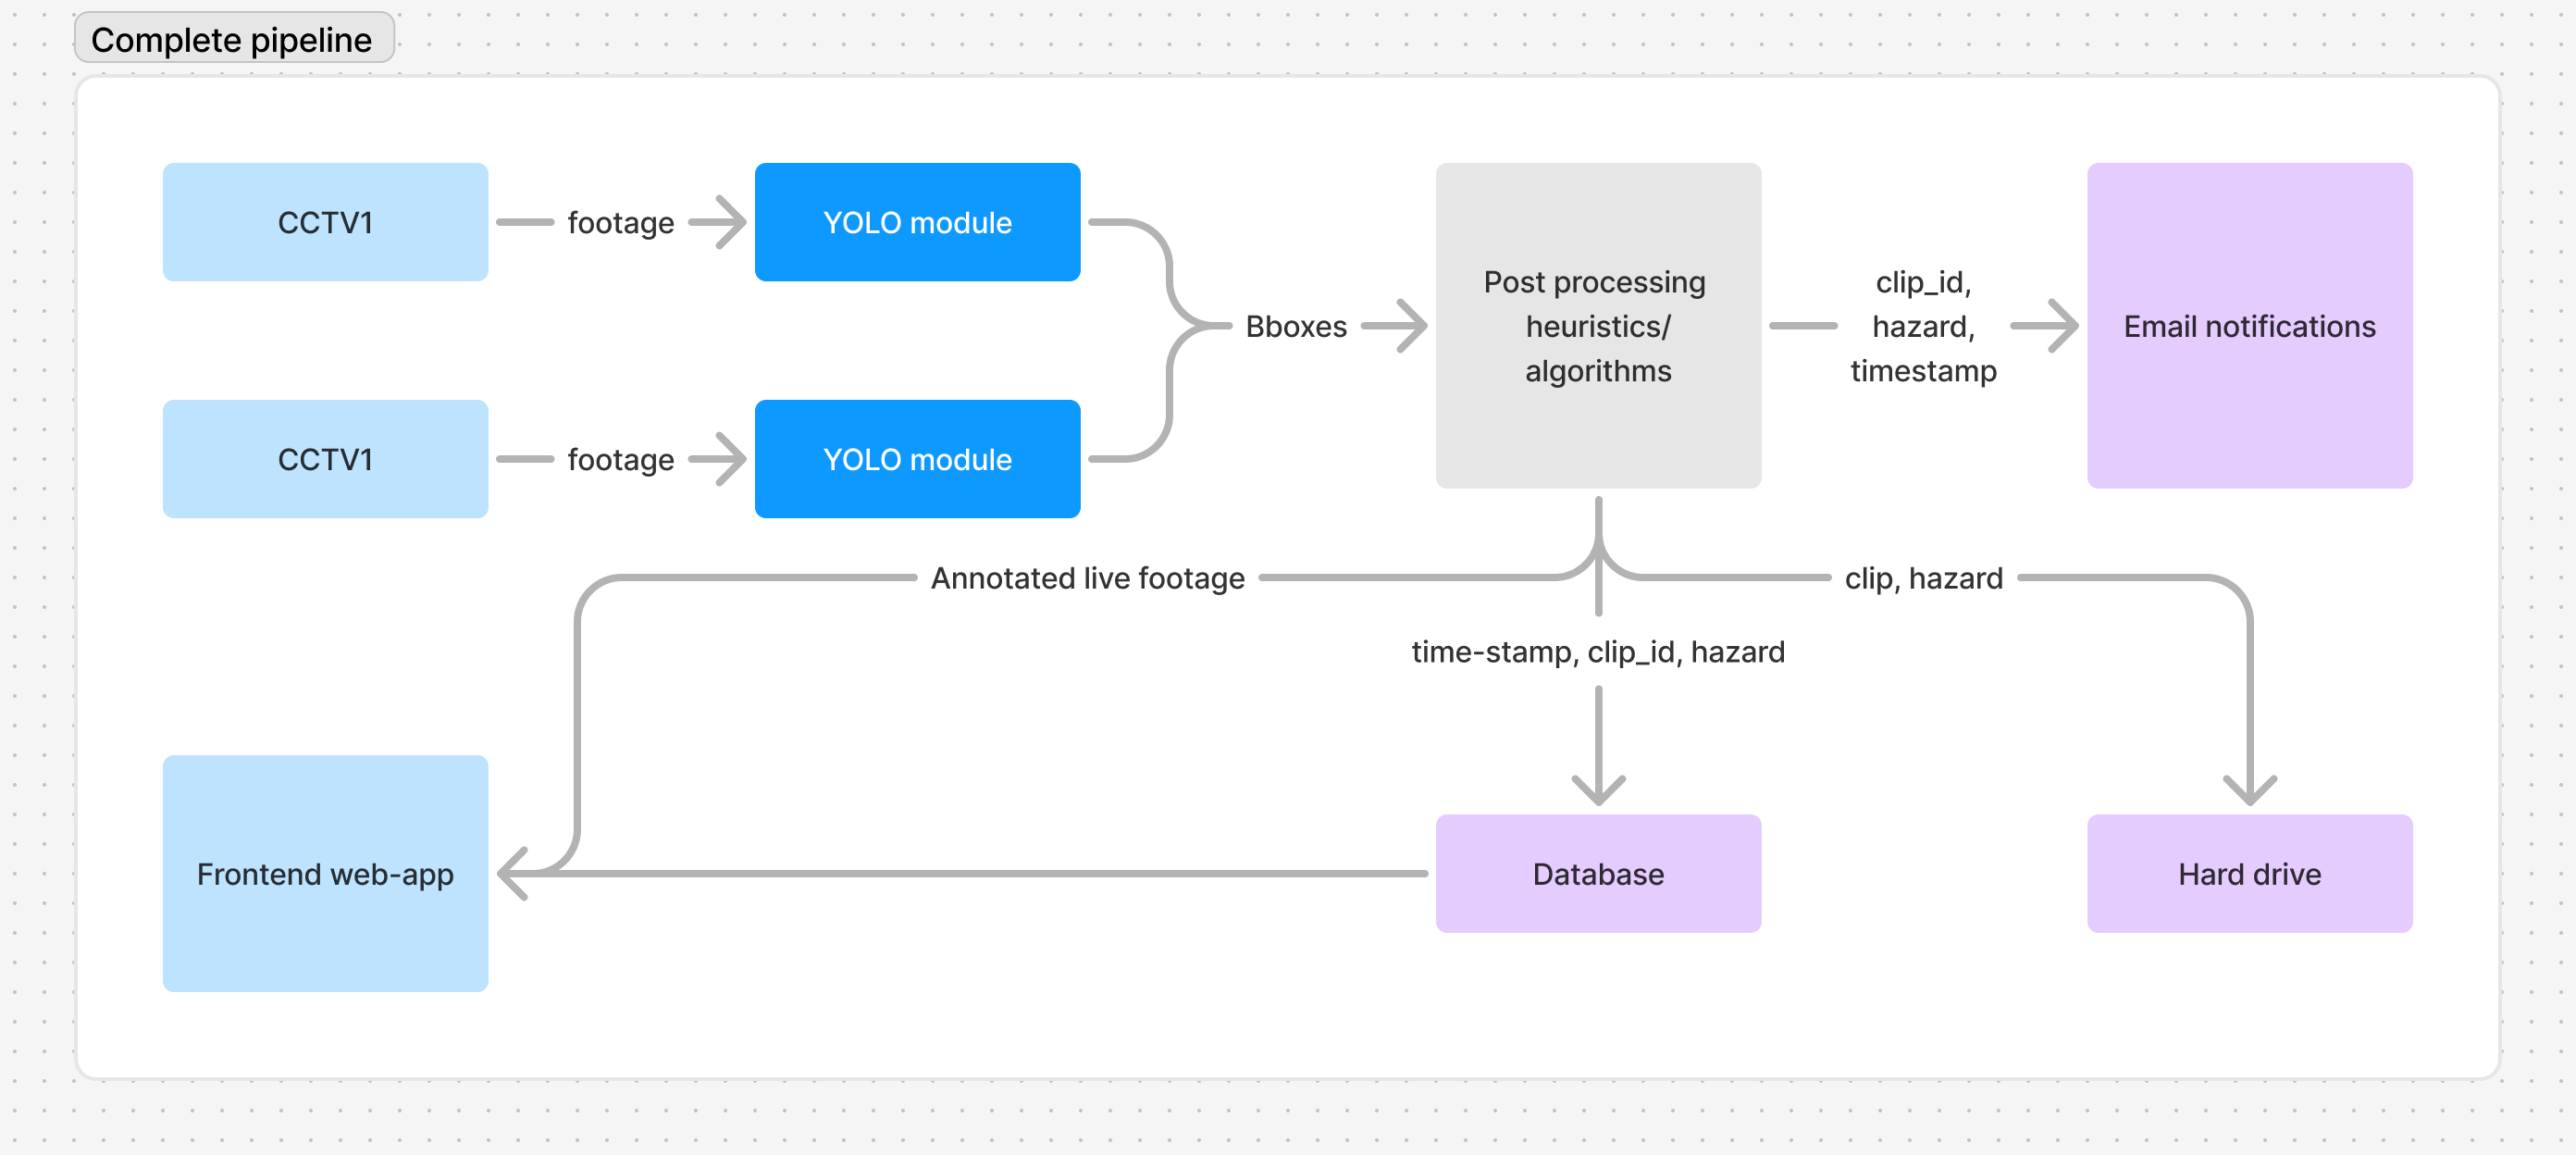
\includegraphics[width=\textwidth]{complete_pipeline.png}
    \caption{Live Data pipeline diagram}
    \label{fig:pipeline2}
\end{figure}

\begin{enumerate}
    \item \textbf{CCTV cameras}: Live video stream from CCTV cameras.
    \item \textbf{YOLO module}: $\leq$4 YOLO models running in parallel, each finetuned for a detection of safety-relevant objects.
    \item \textbf{Post Processing}: Heuristic and non-heuristic algorithms to recognize hazards via relationships of detected objects.
    \item \textbf{Database}: Relational database for statistics and records.
    \item \textbf{Hard drive}: Clips stored locally on server machine.
    \item \textbf{Frontend Web App}: An admin dashboard to look at annotated camera footage and statistics.
\end{enumerate}

\section{Technical Details (20 Points)}
The Technical Details section of our Software Design Specification Document 
will provide a detailed overview of the tools and technologies used in the 
development of the Real-Time Safety Monitoring System and how they will meet 
the requirements specified in the SRS document.
\subsection{Tools and Technologies}
Below are the tools and technologies we are using for the development of this system:
\begin{itemize}
    \item \textbf{Model Finetuning for specific tasks:} PyTorch and CUDA.
    \item \textbf{Model:} YOLOv8 and its finetuned versions for detection tasks.
    \item \textbf{Frontend:} ReactJS (Usage of graph libraries like Chart.js for visualizations).
    \item \textbf{Backend:} Flask.
    \item \textbf{Database:} MSSQL (Usage of relational database for hazard records).
    \item \textbf{Notification Channels:} Email (SMTP-based library: smtplib), SMS (Twilio API).
\end{itemize}

\subsection{Performance Metrics}
Below are the performance metrics for the Real-Time Safety Monitoring System:
\begin{itemize}
    \item Latency: The requirement of a maximum of 5 seconds for hazard detection and alert delivery is planned to be met using asynchronous processing for fast alert delivery, and for the detection part, we plan to use a combination approaches such as usage of optimized YOLO models, model quantization, etc.
    \item Accuracy: The requirement of 85\% minimum detection rate under standard conditions is planned to be met by using deep learning approaches such as addition in dataset using synthetic images generated from GANs, ensemblng, transfer learning, Data Augmentation, Knowledge Distillation, and other techniques.
    \item Frame Rate: We aim to achieve a minimum of 5 frames per second for real-time processing by techniques described in the section about latency optimization.
\end{itemize}

\subsection{Security Features}
We will achieve sound safety protocols by having:
\begin{itemize}
    \item Encrypted communication between components for which we will develop secure APIs, and use HTTPS for web-based communication.
    \item Role-based access controls for user management.
    \item Multi-factor authentication for dashboard login.
    \item Regular security audits and penetration testing (using tools such as Vulert, OWASP ZAP, SonarQube, etc.).
\end{itemize}

\newpage
\section{Conclusion}
In summary, this Software Design Specification document provides a comprehensive blueprint for the design and implementation of the workplace safety monitoring system for Dawlence Pvt. Ltd. It details  the system's architecture, data model, data pipeline, and technical specification and ensures a clear and unified understanding among all stakeholders.
\end{document}
